\subsection{Gaia}
No projeto Gaia foi criado um \emph{middleware} (Gaia OS) com o objetivo de dar suporte ao desenvolvimento e execução de aplicações em \emph{Active Spaces}, ambientes com sistemas interativos. O \emph{middleware}, uma abstração de um sistema operacional, foi projetado para ser uma infraestrutura distribuiída que coordena entidades de software e dispositivos heterogêneos em um \emph{smart space}. O Gaia OS expõe serviços para buscar e utilizar recursos presentes no ambiente, ter conhecimento do contexto e provê um \emph{framework} para desenvolver aplicações móveis sensíveis ao contexto, que conheçam os recursos disponíveis, utilizem múltiplos dispositivos e tenham como foco o usuário~\cite{gaia2002}.

\emph{Active Spaces} são espaços físicos como escritórios, salas de conferência, casas, hospitais, campi universitários, cidades que possuem dispositivos integrados ao ambiente. O objetivo desses dispositivos é prover e obter informação sobre usuários do ambiente, os ajudando a realizar tarefas que eles não poderiam sem os dispositivos, ou facilitando tarefas do cotidiano.

\begin{figure}[ht]
\center
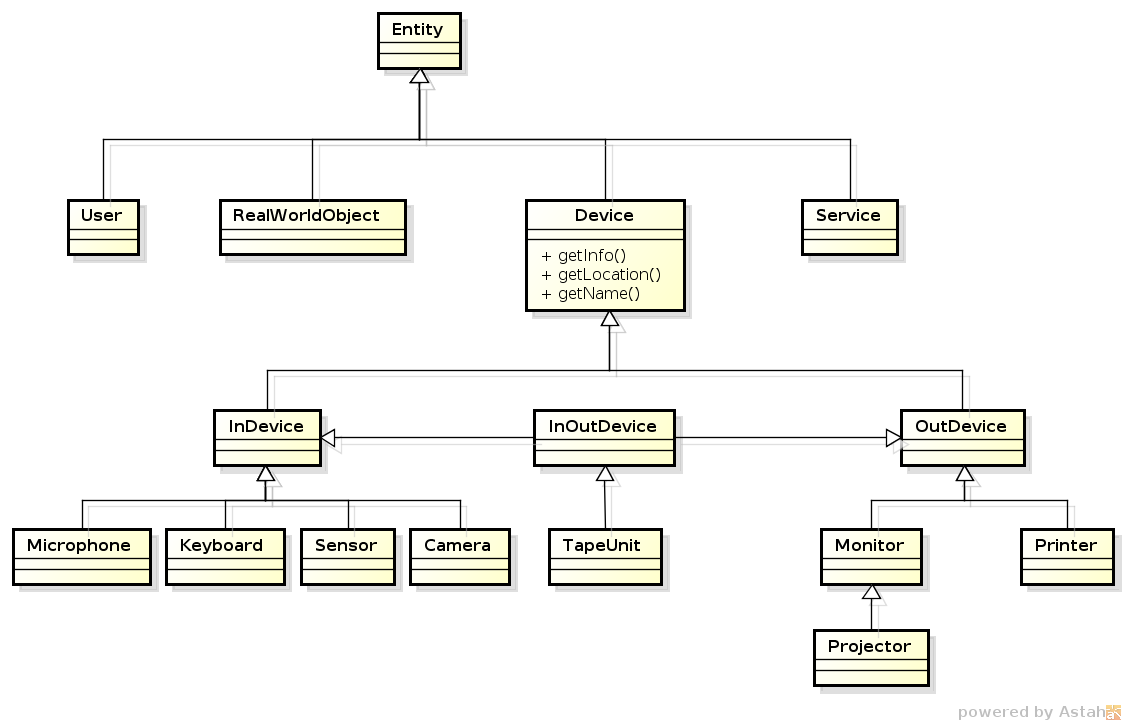
\includegraphics[scale=0.5]{imagens/gaia-devices}
\caption{Diagrama de Classes Simplificado~\cite{gaiaDevices}}
\label{fig:gaiaClassDiagram}
\end{figure}

No projeto, foi desenvolvido um \emph{framework} para a interação entre dispositivos heterogêneos. Esse \emph{framework} permite a representação das interfaces dos dispositivos com diferentes níveis de detalhe e especialização. As interfaces são definidas utilizando IDL(\emph{Interface Description Language}), que permite a construção de \emph{drivers} de dispositivos em qualquer linguagem de programação garantindo uma facilidade de integração com diferentes dispositivos.

A figura~\ref{fig:gaiaClassDiagram} mostra o Diagrama de Classes simplificado do projeto Gaia. Podemos observar que a Classe \emph{Device} é especializada em dispositivos de entrada(\emph{InDevice}) e saída(\emph{OutDevice}) de dados. Os dispositivos de entrada são ainda especializados em: Microfone, Câmera, Teclado e Sensor, enquanto os dispositivos de saída são especializados em: Impressora e Monitor, que por sua vez, é especializado em Projetor. Há ainda a interface para dispositivos que são de entrada e saída que é especializada em uma unidade de Fita.

\begin{comment}
http://gaia.cs.uiuc.edu/html/device.htm
http://gaia.cs.uiuc.edu/papers/GaiaSubmitted3.pdf
\end{comment}
